\documentclass[spanish]{udpreport}
\usepackage[utf8]{inputenc}
\usepackage[spanish]{babel}

% Podemos establecer el logo de alguna entidad o dejar el de la UDP (defecto)
%\setlogo{EITFI}

\title{Informe de redes de datos 8\\
"SOCKET": Implementación de juego para redes de datos\\}
\author{Alumno: Camilo Araya
\\Profesor: Nicolás Hidalgo\\Ayudante: Martín Griño}
\date{\today}



\begin{document}
\maketitle

\chapter*{Resumen} 
\addcontentsline{toc}{section}{Resumen} 
\markboth{RESUMEN}{RESUMEN} 
en el presente informe se abordara una breve explicación de como se logro implementar la 
funcionalidad de un juego que sigue con la dinámica del  Ping-pong el cual 
fue modelado para dos personas, esto se logro 
 mediante la implementación de sockets a través de dos
programas se logre establecer una comunicación entre si, para esto se ha procedido al uso e
implementación de dos lenguajes de programación mas usados para este proyecto.
\\En este proyecto se logra demostrar con hechos la funcionalidad de Sockets y parte de sus usos, en otros términos el desarrollo de videojuegos, chats y otros son posibles gracias a este mecanismo.
\tableofcontents
\chapter{Introducción}
Un socket es una dirección de Internet que funciona combinando una dirección IP correspondiente
 a la dirección numérica única de cuatro dígitos que identifica a un dispositivo particular 
en la red, junto con un número de puerto correspondiente al número que identifica
 una aplicación de una red en particular.
 \\[0.2cm]
Una manera de implementar de forma visual una programación orientada a sockets es mediante la 
creación de juegos o un checksum, forma en que podremos ver como realmente se le da sentido 
a  los contenidos informativos de redes de datos.
\\[0.2cm]
Un socket a grandes rasgos  cumple con la definición de conector pero no eléctrico si no que mas
bien a niveles de redes e internet, a continuación se enumeraran los tópicos abordados para la elaboración del proyecto.
\\[0.2cm]
\section{HTML}
 Lenguaje de programación de hipertexto orientado netamente a la elaboración de paginas web.
\\[0.2cm]
\section{SOCKET}
 Es netamente orientada a las conexiones, se garantiza una transmisión
de todos sus octetos sin errores ni omisiones y garantiza que todos sus octetos
llegan a su destino en el mismo orden que fue transmitido.
\\En otras palabras Sockets establece un enlace entre dos programas que se ejecutan de manera independiente uno del otro, generalmente se da entre programa cliente y programa servidor.
\\[0.2cm]
\section{JAVA SCRIPT}
Lenguaje de programación con el cual se podrá realizar (client-side) y (server-side) y así poder dar la dinámica al programa que se quiera ejecutar.
\\[0.2cm]
\chapter{Implementación y montaje}
Para la implementación preliminar del juego de Ping-pong el que fue seleccionado para presentar como proyecto, este fue programado en JavaScript planteado para dos jugadores, el resultado obtenido se vería algo así como la siguiente imagen:
\begin{figure}[h]
    \centering
    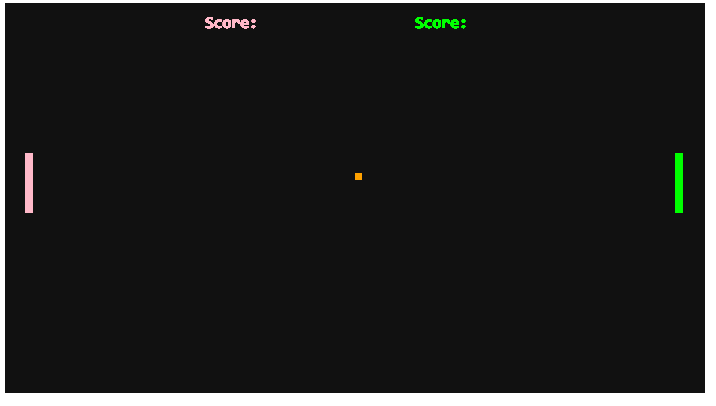
\includegraphics[scale=0.5]{images/juego.png}
    \caption{Visión preliminar del Juego}
    \label{fig:my_label}
\end{figure}
\\ Uno de los puntos más fuertes  y a su vez más complejos de la implementación de dicho juego fue el movimiento de los jugadores y el movimiento de la pelota ya que había que definirlo. Otros aspectos que se hicieron en base a la estética del juego fue asignarle colores o también cambiar las dimensiones de los jugadores los cuales fueron un plus al momento de modelar el juego. 
\newpage En cuanto al modelo propuesto por sockets para poder ejecutar el juego se estableció para cliente-servidor con un único TCP. La librería Sockets.io permitió que el juego modelado tuviera interacción para multi-jugarores,  
\begin{figure}[h]
    \centering
    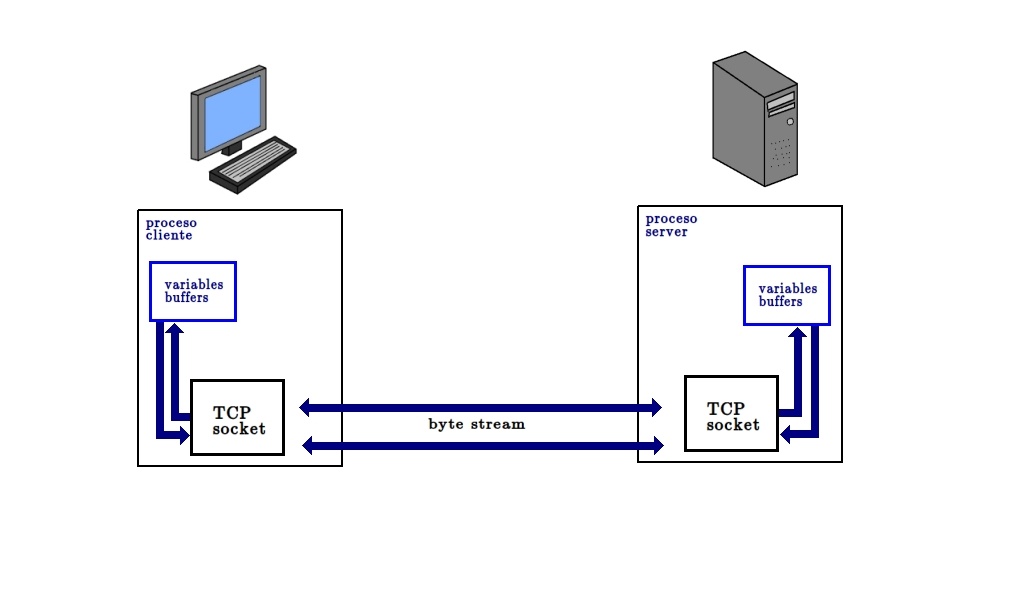
\includegraphics[scale=0.5]{images/sock.jpeg}
    \caption{Funcionamiento}
    \label{fig:my_label}
\end{figure}
\\[0.5cm] El uso de HTML en la implementación se requirió para poder establecer conexiones para multi-jugadores de forma independiente con ayuda de Sockets, junto con esto una de las grandes ventajas es que al abrir los navegadores en la URL se podrá ver la actualización de cada movimiento que se haga es instantánea. 
\\[9cm]
\textbf{El funcionamiento del programa serán expuestos en la presentación correspondiente.}
\chapter{Conclusión}
Se concluye del presente informe que en base a los conceptos vistos en el ramo redes de datos, este trabajo ilustra de forma tangible el funcionamiento de redes y como se pueden establecer conexiones de dos dispositivos enlazándolos. Sockets fue muy util para establecer la conexión de el juego de Ping-pong modelado para este proyecto ya que se pudo ver que dos jugadores de forma independiente pueden interactuar sobre el mismo programa.



\begin{thebibliography}{0}
\bibitem{1}http://codigoprogramacion.com/cursos/java/103-sockets-en-java-con-cliente-y-servidor.html#.Wg-CTrT1VE4 \\ 
\end{thebibliography}
\listoffigures
\end{document}

